\documentclass[11pt, a4paper]{article}
\usepackage[utf8]{inputenc}
\usepackage[left=2.35cm, right=3.35cm, top=3.35cm, bottom=3.0cm]{geometry}
\usepackage{amsmath, amssymb, amsthm}
\usepackage[english]{babel}
\usepackage{graphicx}
\usepackage[font={small,it}]{caption}
\graphicspath{ {figures/} }
\usepackage{url}
\usepackage{appendix}
\usepackage{float}
\usepackage[bottom]{footmisc}
\usepackage{titling}
\setlength{\droptitle}{-10em}  

\title{ \huge Artificial neural networks \\ 
  { \large Assignment 1: Supervised learning and generalization }}
\author{
        Lood, Cedric \\
        \small Master of Bioinformatics
}

\begin{document}
\maketitle
%\tableofcontents

\section{Context}

Artificial neural networks that have at least 1 hidden layer have the
property of being universal
approximator\cite{hornik1989multilayer,leshno1993multilayer}. Hence,
any non-linear function can be realized using classical feedforward
multilayers networks. In this assignment, we were asked to explore the
different training algorithms that can be used with backpropagation in
order to learn non-linear functions. These function have different
yields in terms of performance, training time, and more importantly
generalization. Some comparisons of the approaches are explored in
this report.

\noindent For illustration purposes, I worked with 2 functions
illustrated here (graphics created using ggplot2 and R \footnote{All
  matlab and R code can be found online at:
  https://github.com/milt0n/ANN-Experiments}):

\begin{itemize}
\item A simple polynomial function with equation $f(x)=x^3-11x+2$
  illustrated on the left of figure \ref{fig:functions}.
\item A more \emph{``wiggle-y''} function, that exhibits some
  dampening, with equation $g(x)=e(-x^2)sin(10x)$ illustrated on the
  the right of figure \ref{fig:functions}.
\end{itemize}

\begin{figure}[H]
    \centering
    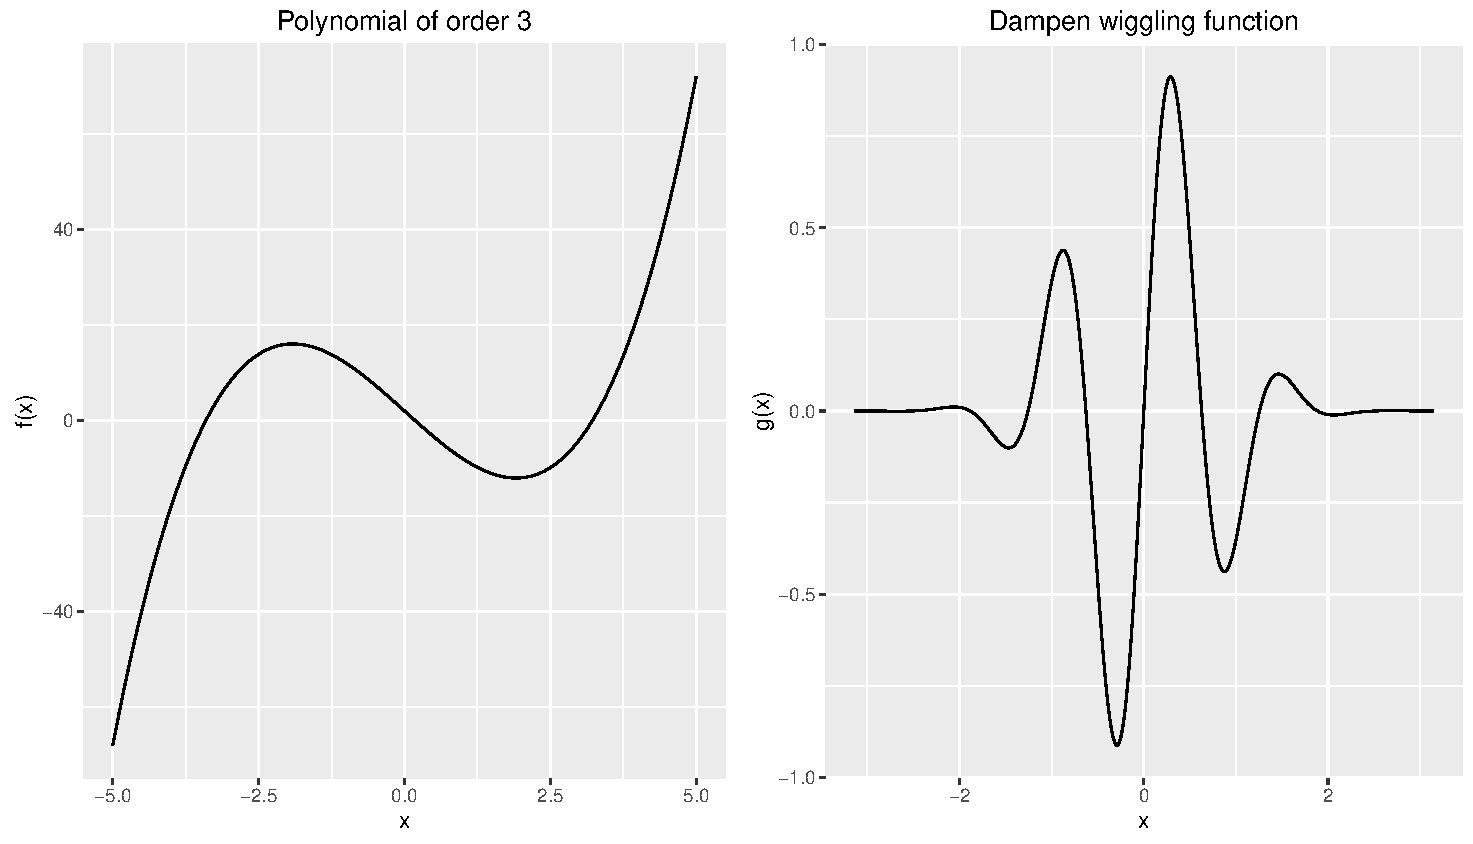
\includegraphics[scale=.50]{true_functions.pdf}
    \caption{Graphs of the underlying true functions used in the analysis}
    \label{fig:functions}
\end{figure}

\section{Noise-free learning}
In this section, we explore the learning in a supervised manner of a
dataset produced by a known underlying function. The entry for the
learning algorithm is thus a set of tuples $(x, y)$ with $x$ chosen
over a given interval, and $y=f(x)$.

The architecture chosen for the feedforward multilayer neural net
consisted of 1 hidden layer, with 10 neurons, and 1 neuron in the
output layer. The transfer function for the hidden layer neurons is
the sigmoid, and the output neuron has a linear transfer function
$f(x)=x$. On figure \ref{fig:traingd}, one can see that the training
of the neural net using gradient descent (\emph{traingd} in matlab):

\begin{description}
\item [top graph] that represents the polynomial function
  $f(x)=x^3-11x+2$. This performed originally the worst, with a
  problem of computation of the gradient during the training. The
  gradient at each \emph{epoch} of the training becomes larger and
  larger, and eventually too large to represent (\emph{NaN} in matlab)
  after only 50 \emph{epochs}. After investigation, the problem seemed
  to lie in the variance of the target function, which was too large
  for the gradient descent algorithm. I found a solution to that
  problem that involved rescaling the function's variance using the
  \emph{zscore} function in matlab.
\item [bottom graph] the gradient descent performed without problems
  on $g(x)=e(-x^2)sin(10x)$ but the performance were still not
  satisfying in terms of approximation. I tried raising the number of
  \emph{epochs} to 10000 and 100000 (not shown on the graph), which
  takes significantly more time to compute, but it did not result in
  any significant increase in the quality of the fit.
\end{description}

\begin{figure}[H]
  % \centering
  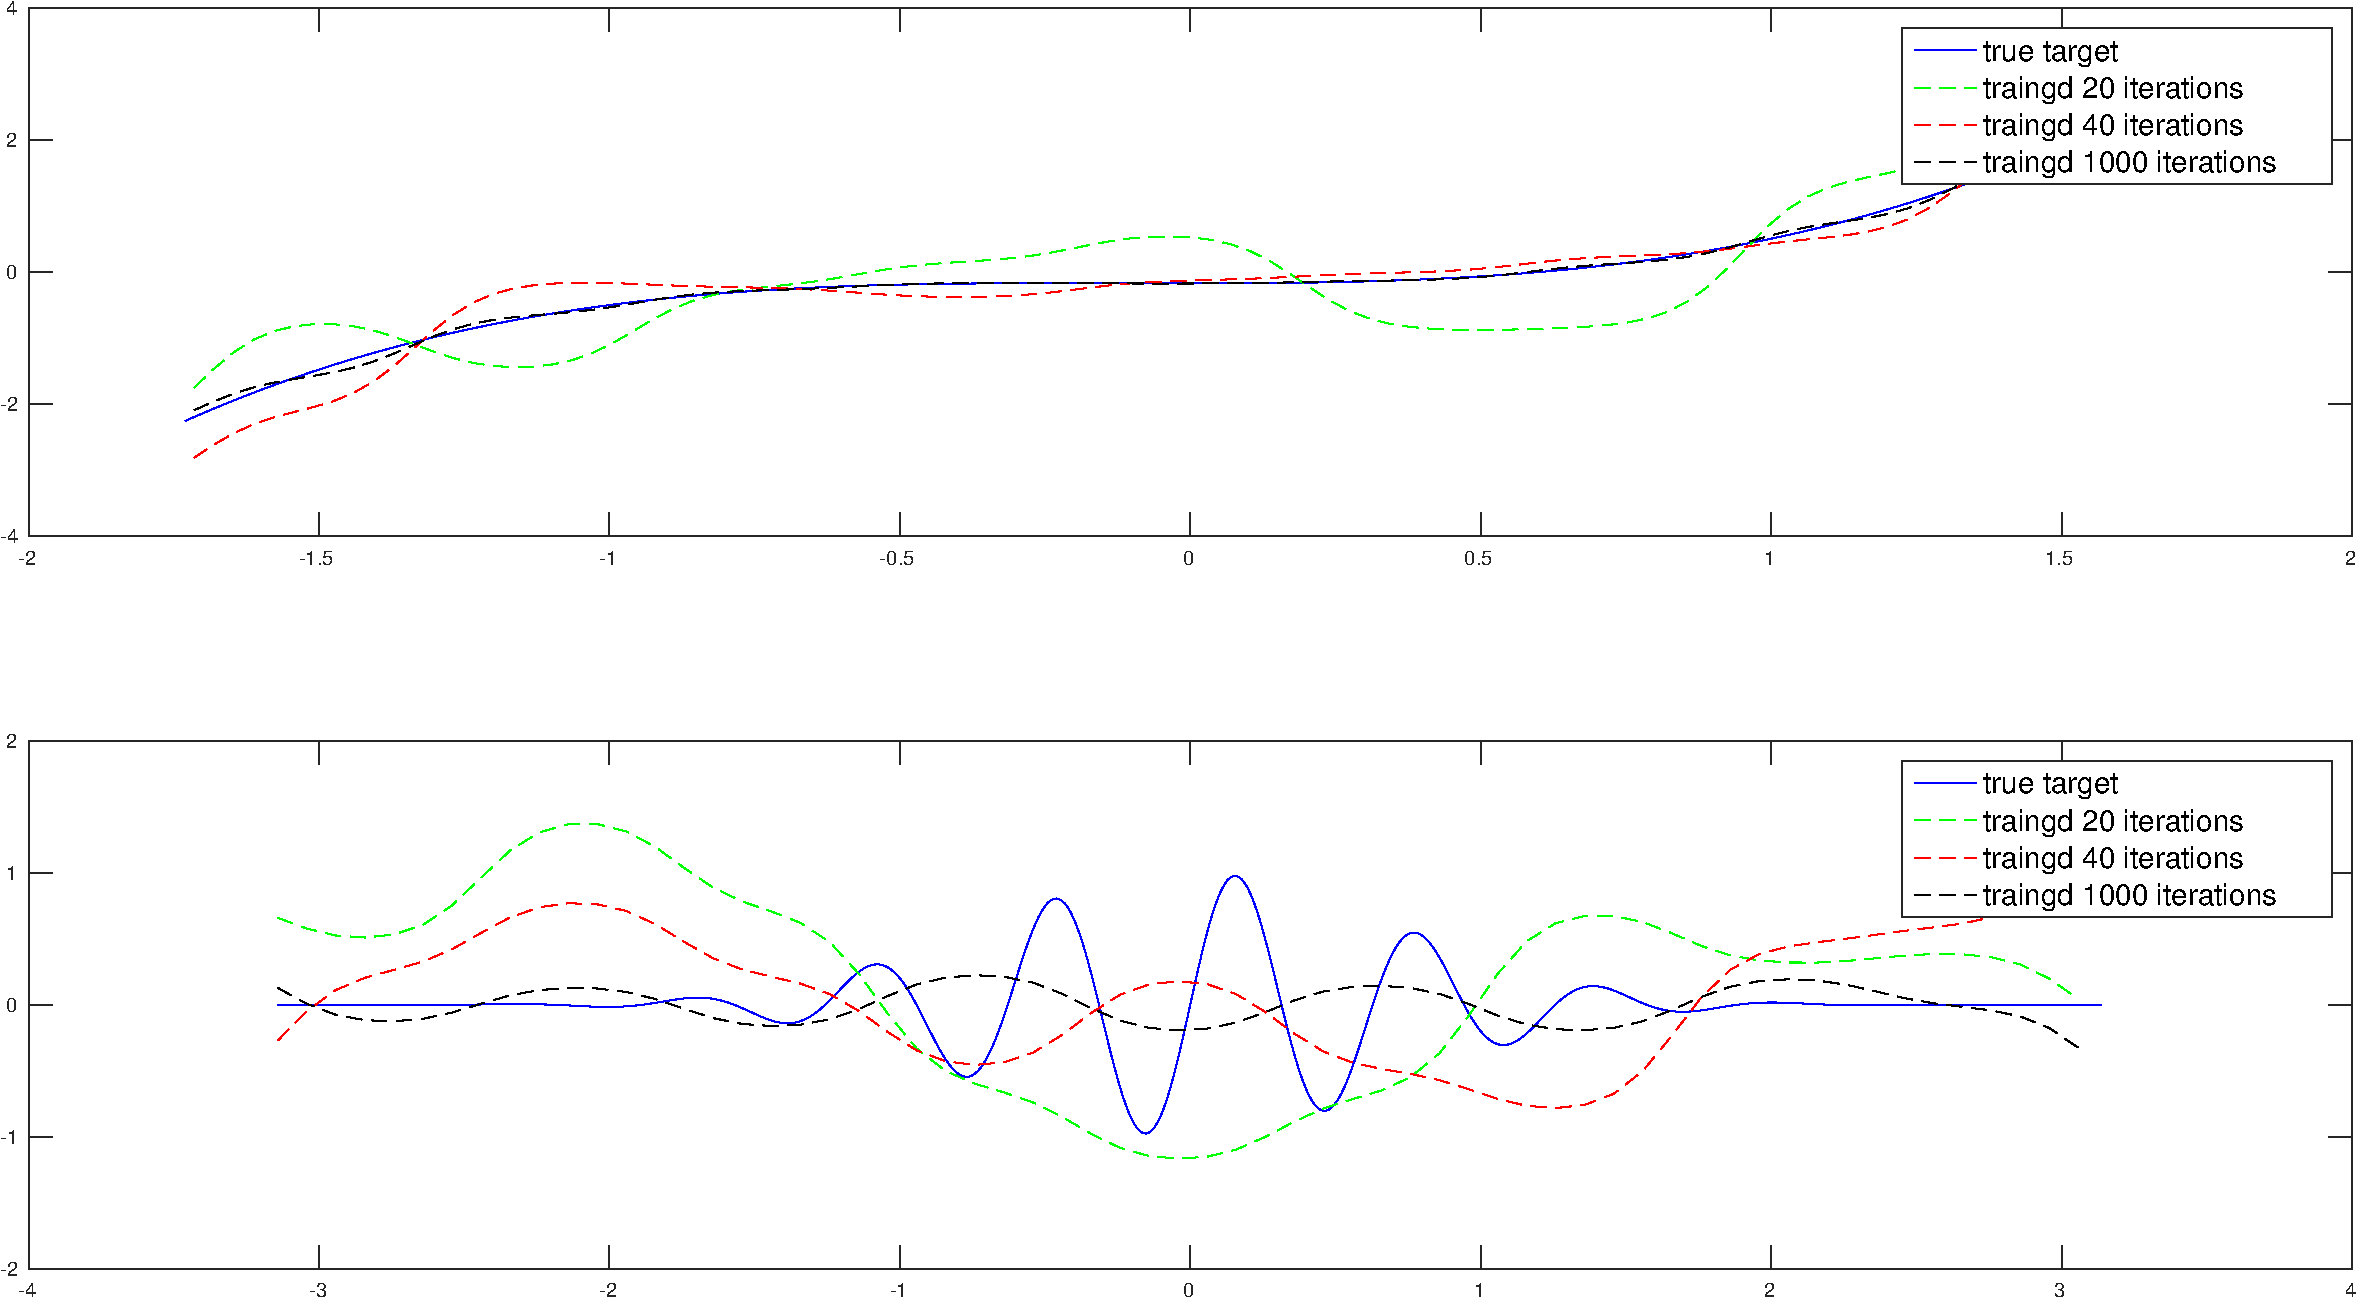
\includegraphics[scale=.43]{traingd.pdf}
  \caption{Training with gradient descent}
  \label{fig:traingd}
\end{figure}

Training with Levenberg-Marquardt backpropagation methods worked
really well with the 2 functions. The results in terms of fitting and
performance are illustrated in \ref{fig:trainll}. Only a few
iterations of the training algorithm were required to fit the
polynomial function $f(x)=x^3-11x+2$. At most 10 iterations were
sufficient to obtain a $R^2$ of 1 for the model.

The function $g(x)=e(-x^2)sin(10x)$ took an order of magnitude more
steps to obtain such a satisfying fit (with an $R^2$ of 1).

\begin{figure}[H]
  % \centering
  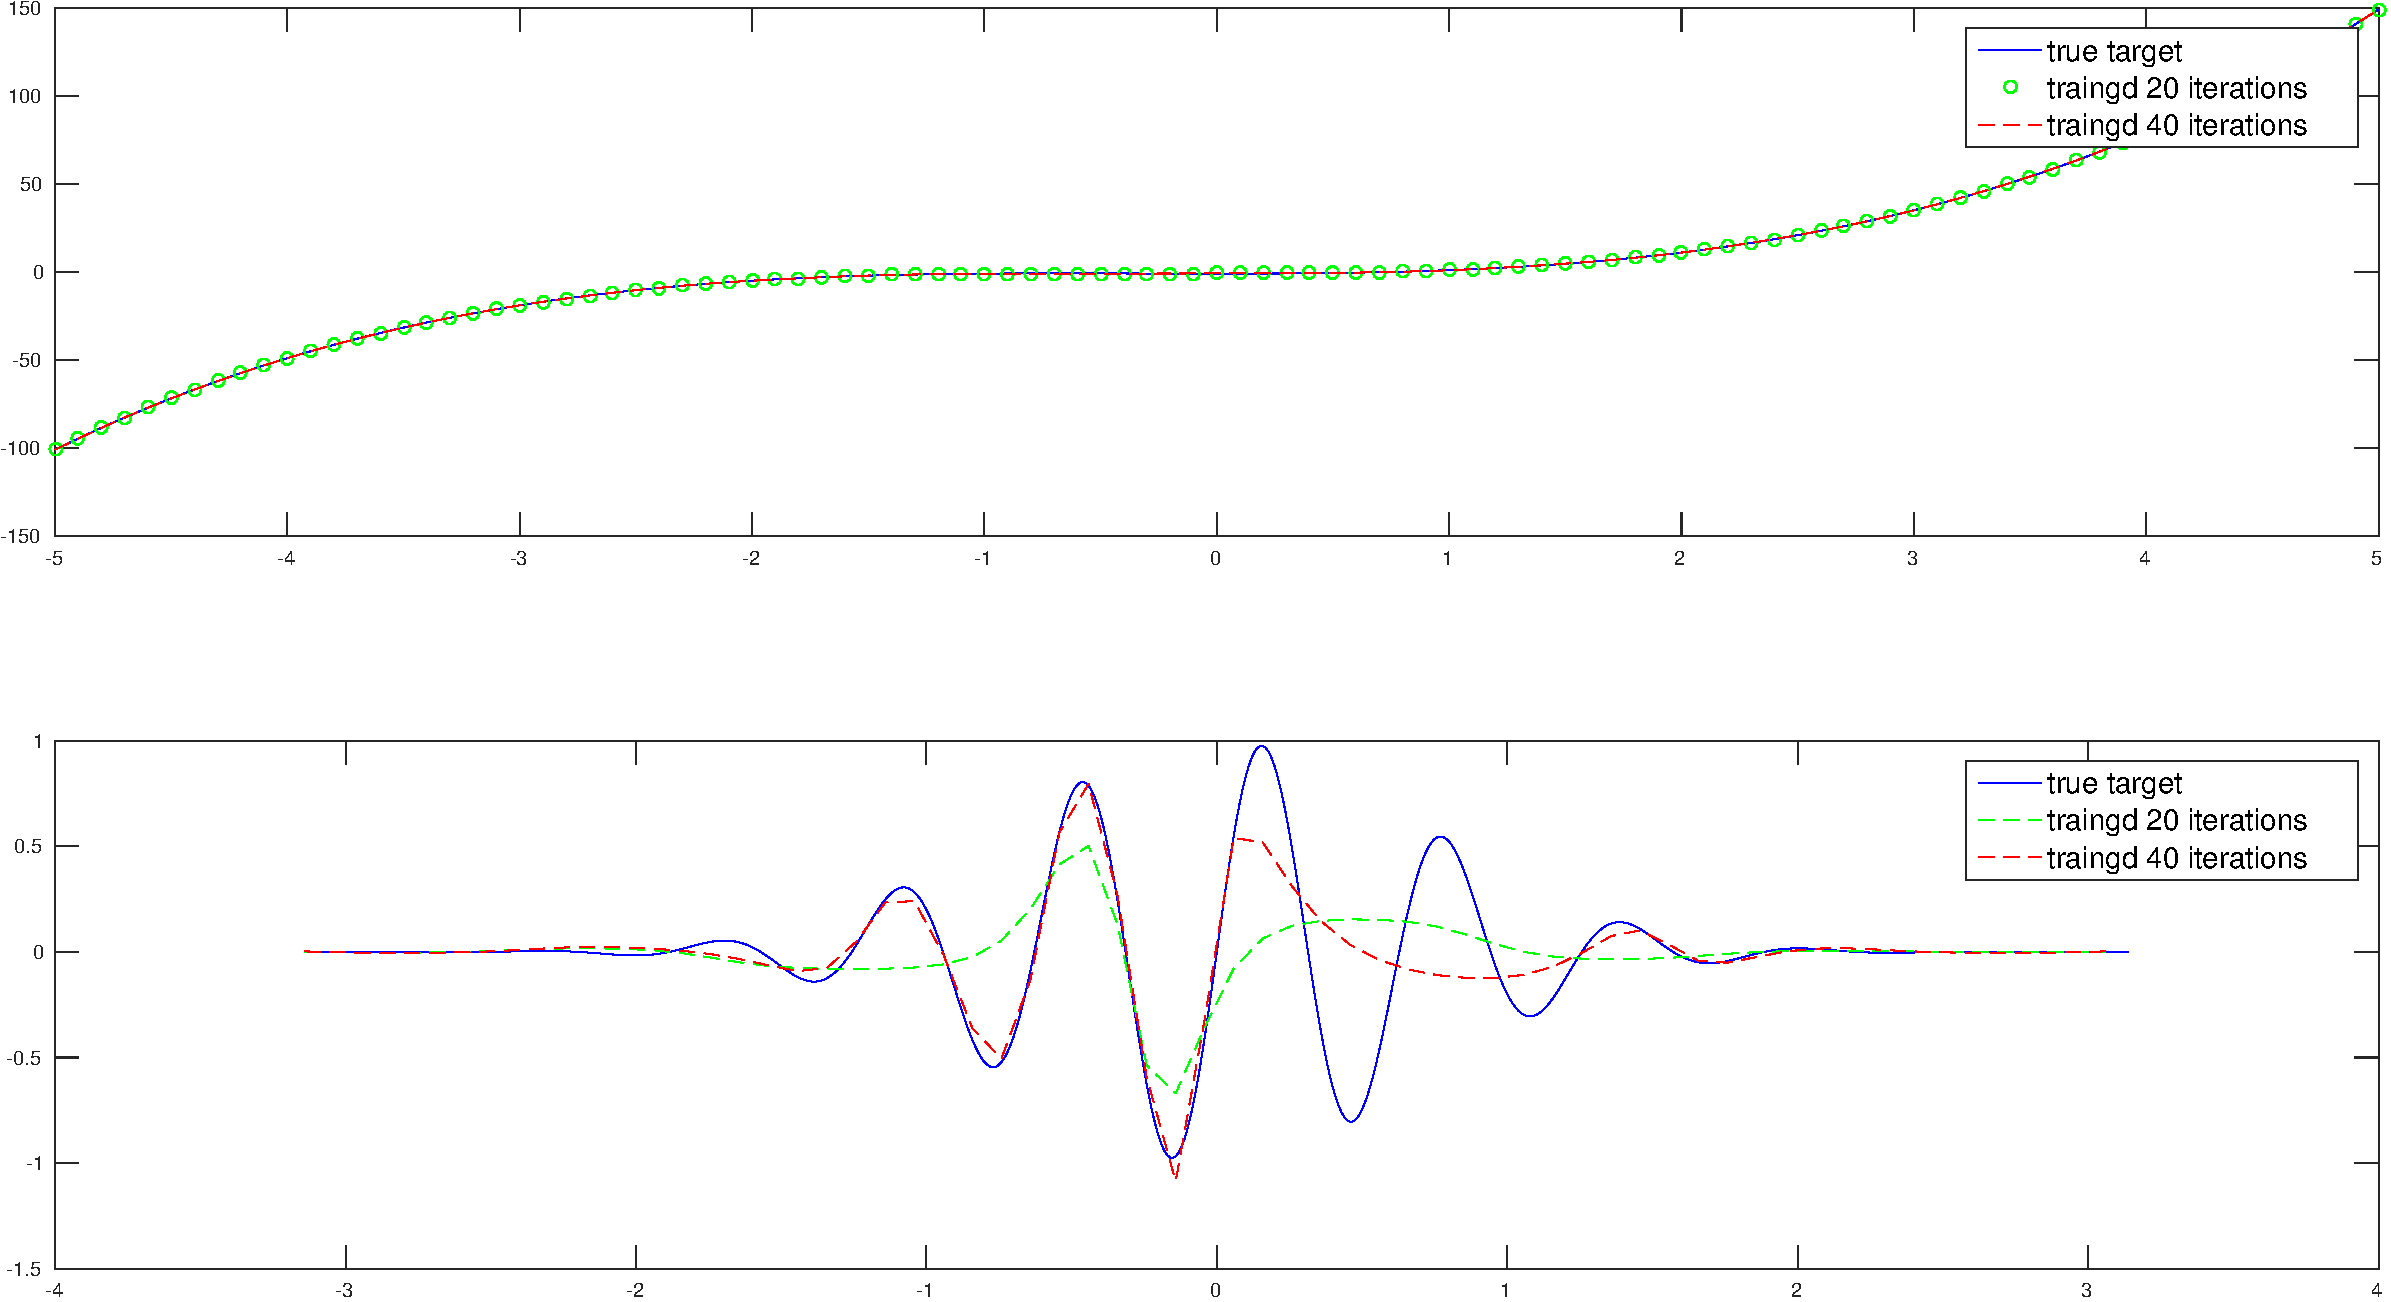
\includegraphics[scale=.43]{trainlm.pdf}
  \caption{Training with Levenberg-Marquardt backpropagation}  
  \label{fig:trainll}
\end{figure}

\section{Learning in noisy setting}

To simulate the presence of noise in the dataset, I chose to add a
normally distributed $\epsilon$ to $f(x)$, for example:
$f_{noisy}=f(x)+N(0,1)$. 

See graphic \ref{fig:trainnoise} where the noisy dataset was used for
training. Typical overfitting can be seen when raising the value of
the \emph{epochs}, represented in the graph by the red curve, which
upon closer inspection seems to be following the noise rather than
fitting the underlying function. Strategies to decide when to stop
training can be implemented, such as validation set, cross validation,
and bootstrapping.

\begin{figure}[H]
  % \centering
  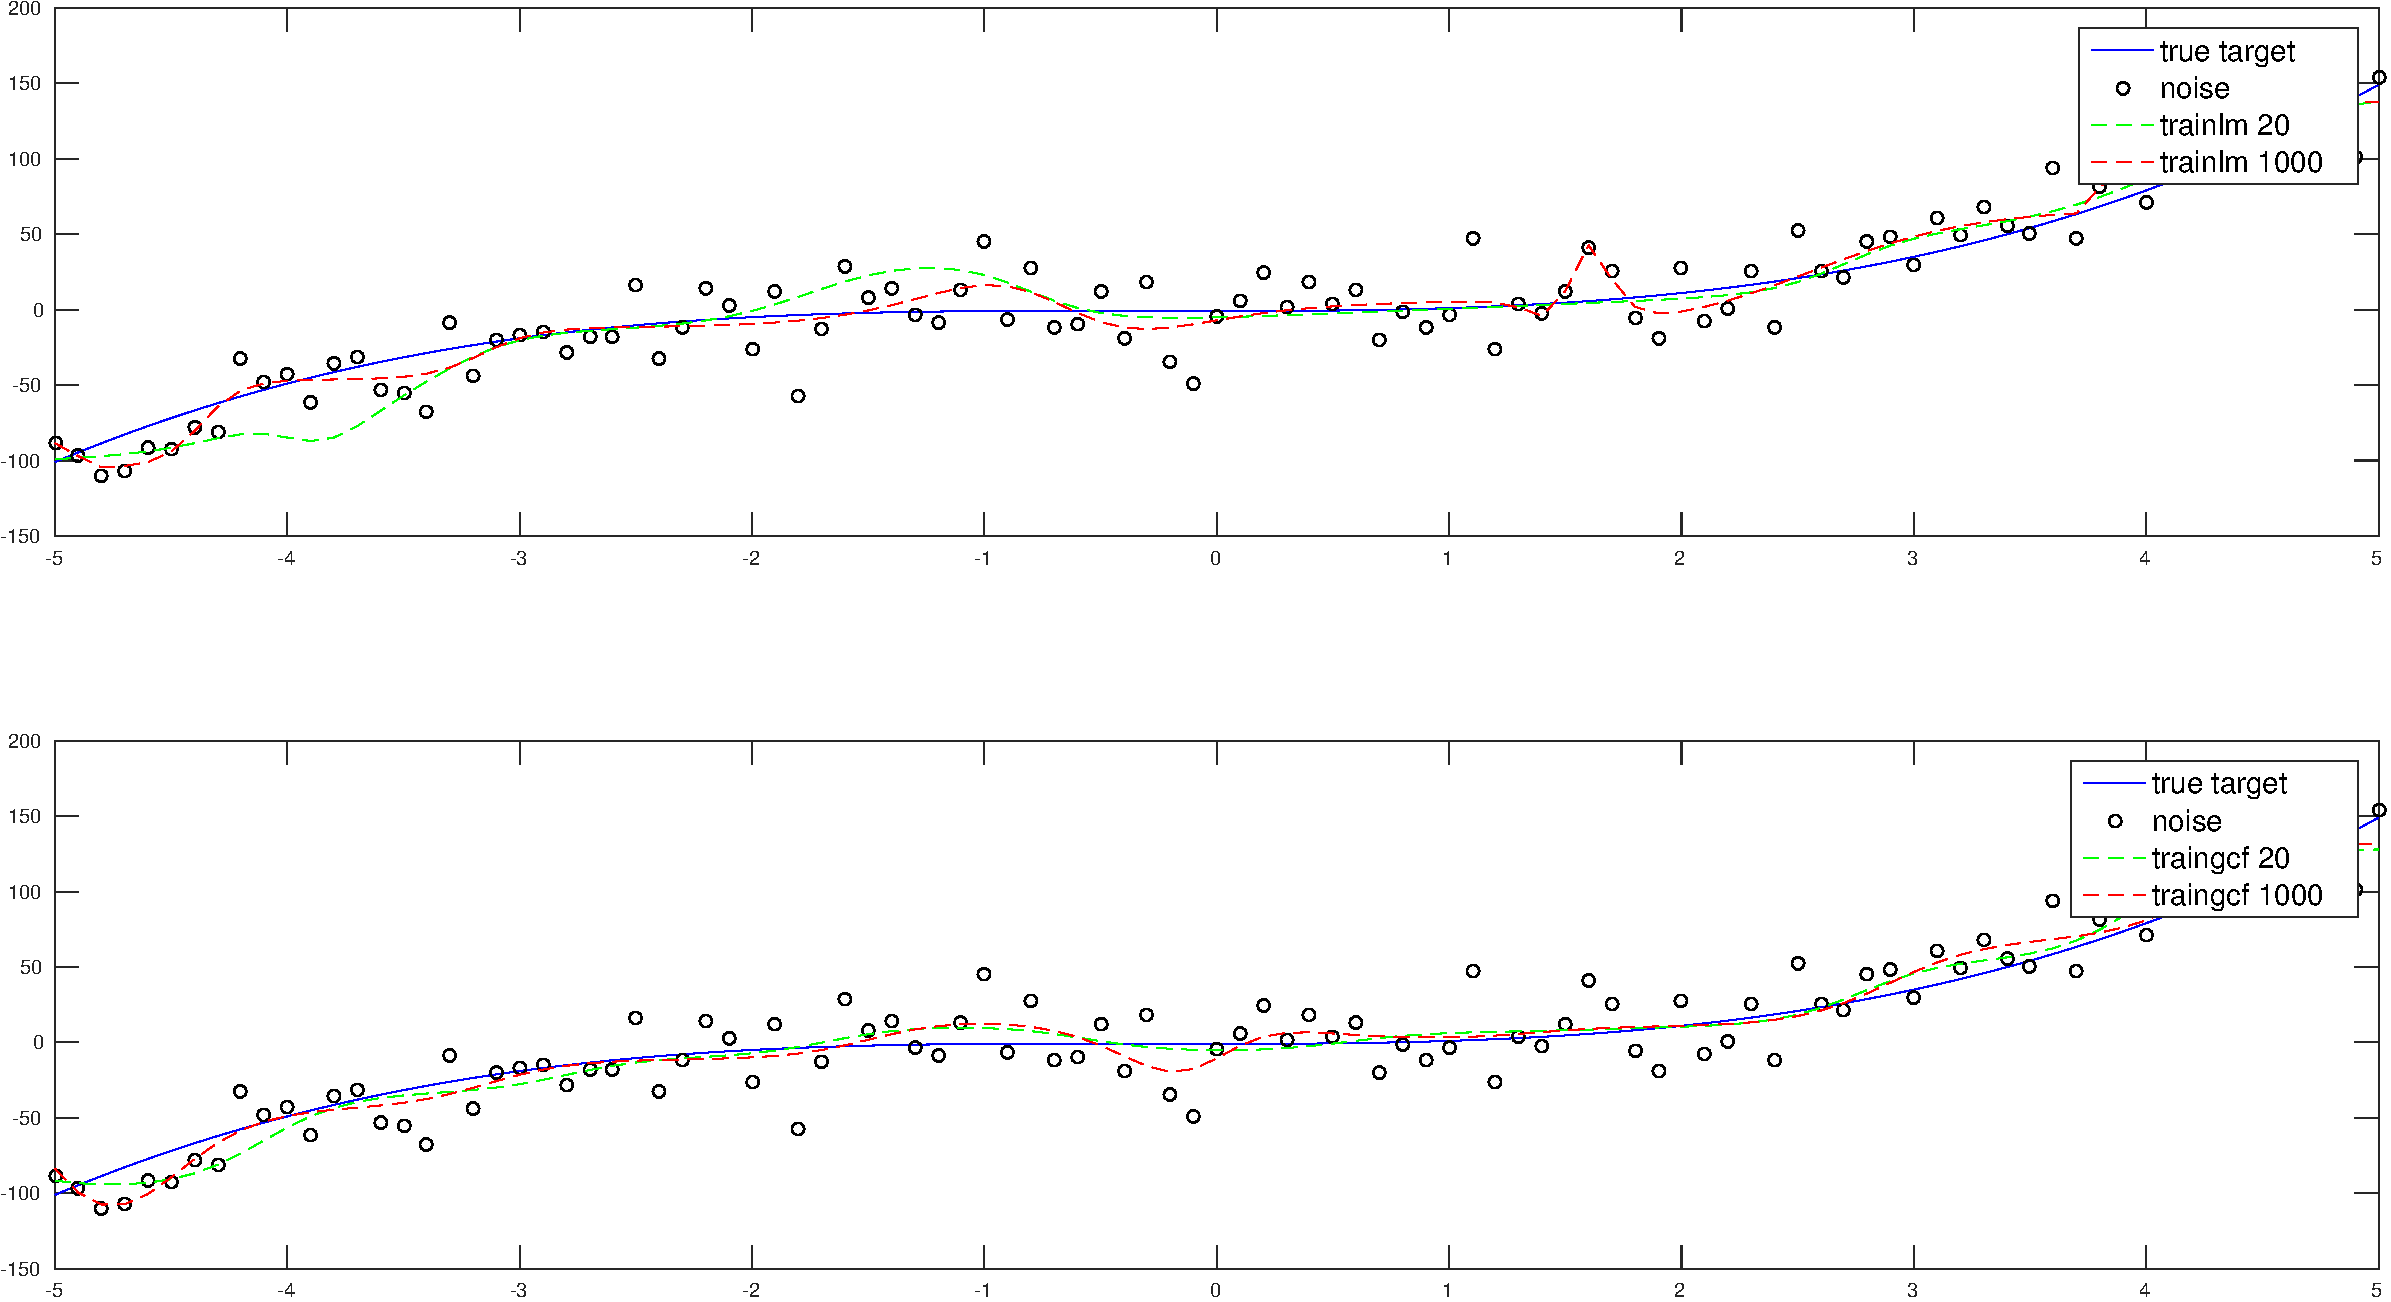
\includegraphics[scale=.43]{trainnoise.pdf}
  \caption{Example of overfitting in noisy dataset}  
  \label{fig:trainnoise}
\end{figure}

\section{Perspectives}

A couple of observations and insights were gained doing this analysis. 

\begin{itemize}
\item the stochasticity of the process of training was really visible
  in the results. Some of the neural networks did fit the data almost
  to perfection on some of the training (as can be surveyed using the
  $R^2$ variable available through \emph{postregm}), only to perform
  poorly during another round of training with the same
  settings. Setting a seed value solved that variation, but it is an
  interesting observation nonetheless.
\item in general, gradient descent performs terribly in terms of
  fitting noiseless, known underlying function. Training with
  Levert-Maquart yielded the best performance overall.
\end{itemize}

\bibliographystyle{ieeetr} 
\bibliography{bib-db}

\end{document}
